\documentclass[a4paper, 11pt, twocolumn]{article}

\usepackage[a4paper, total={6.24in, 8.5in}]{geometry}
\usepackage[utf8]{inputenc}
\usepackage{graphicx}
\usepackage{verbatim}
\usepackage{float}
\usepackage{array}
\usepackage{xfrac}
\usepackage{mathpazo}
\usepackage{amsmath}
\usepackage{bm}
\usepackage{multirow}
\usepackage{makecell}
\usepackage{multicol}
\usepackage{sectsty,textcase}
\usepackage{wrapfig,lipsum,booktabs}
\usepackage{enumitem}
\usepackage{hyperref}
\usepackage{makecell}
\usepackage{array}
\usepackage{layouts}

\bibliographystyle{plain}
\renewcommand{\thesection}{\arabic{section}}
\setlength{\columnsep}{15pt}
\newcommand{\myparagraph}[1]{\paragraph{#1}\mbox{}\\}

\title{FYS-STK3155/4155 Applied Data Analysis and Machine Learning - Project 3 }

\author{Lotsberg, Bernhard Nornes \\ Nguyen, Anh-Nguyet Lise \and
\url{https://github.com/liseanh/FYS-STK4155-project3}}
\date{November - December 2019}
\begin{document}
\twocolumn[
  \begin{@twocolumnfalse}
    \maketitle
    \begin{abstract}
		Whole page: \printinunitsof{in}\prntlen{\textwidth}
		Column: \printinunitsof{in}\prntlen{\columnwidth}
	\end{abstract}
  \end{@twocolumnfalse}
]


\section{Introduction}
In popular culture the neural network is probably the most well known form of 
machine learning. In recent years many other statistical learning methods have 
proven themselves as well however. In this project we compare the performance of 
neural networks and gradient boosting in the case of binary classification.
In addition to these, we also use the much simpler k-nearest neighbours method 
as a baseline for classification performance.



\section{Data}

The data set we will analyse in this project is the MAGIC Gamma Telescope data
set retrieved from the \href{https://archive.ics.uci.edu/ml/datasets/MAGIC+Gamma
+Telescope}{UCI Machine Learning Repository}, which was generated by a Monte
Carlo (MC) program described by D. Heck et. al. \cite{heck1998corsika} to
simulate high energy gamma particle registration in a Cherenkov gamma telescope.
The set consists of ten explanatory variables and a binary response variable
\texttt{class} which specifies whether the measured photons resulted from a gamma
particle (\texttt{class} = g) or a hadron (\texttt{class} = h). The entire data
set consists of 19020 instances with no missing values, with outcome distribution
as shown in Figure \ref{fig:Histogram}. The explanatory and response variables
are defined as the following by the UCI Machine Learning Repository
\cite{Dua:2019}:

\begin{enumerate}[leftmargin=5mm, itemsep=0pt,  parsep=1pt]
  \item \texttt{fLength}: continuous \# major axis of ellipse [mm]
  \item \texttt{fWidth}: continuous \# minor axis of ellipse [mm]
  \item \texttt{fSize}: continuous \# 10-log of sum of content of all pixels
        [in \#phot]
  \item \texttt{fConc}: continuous \# ratio of sum of two highest pixels over
        \texttt{fSize} [ratio]
  \item \texttt{fConc1}: continuous \# ratio of highest pixel over \texttt{fSize} 
        [ratio]
  \item \texttt{fAsym}: continuous \# distance from highest pixel to center,
        projected onto major axis [mm] 
  \item \texttt{fM3Long}: continuous \# 3rd root of third moment along major
        axis [mm] 
  \item \texttt{fM3Trans}: continuous \# 3rd root of third moment along minor
        axis [mm] 
  \item \texttt{fAlpha}: continuous \# angle of major axis with vector to origin
        [deg] 
  \item \texttt{fDist}: continuous \# distance from origin to center of ellipse 
        [mm] 
  \item \texttt{class}: g, h \# gamma (signal), hadron (background)
\end{enumerate}


\begin{figure}
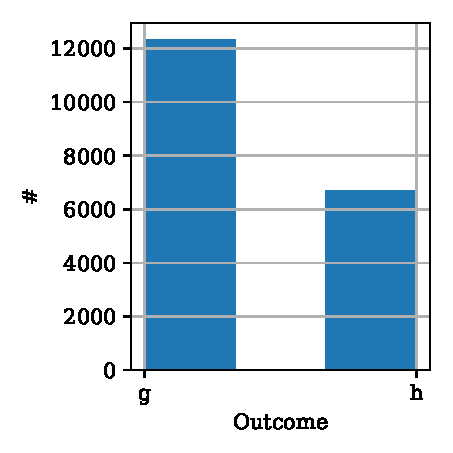
\includegraphics[scale=1]{{figures/histogram}.pdf}
\caption{Frequencies of the outcomes g and h in the data set. The numbers of
instances for the categories were 12332 and 6688 for g and h respectively.}
\label{fig:Histogram}
\end{figure}

\begin{figure*}
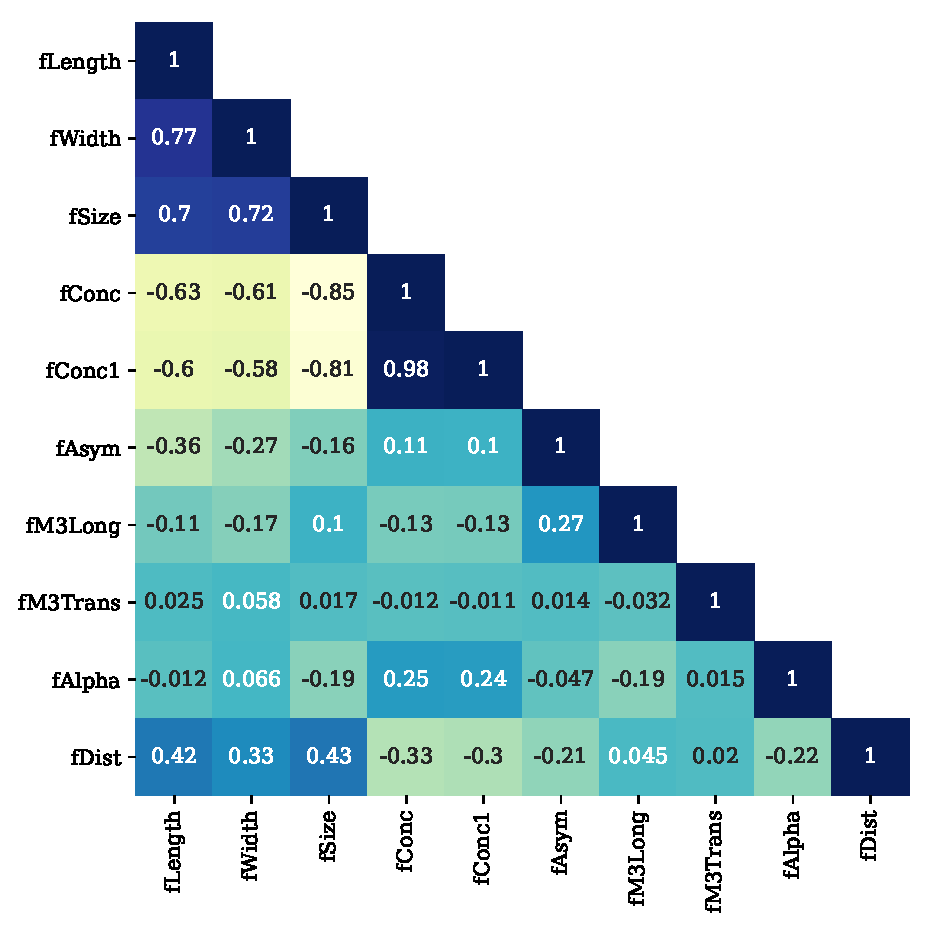
\includegraphics[scale=1]{{figures/correlation_matrix_train}.pdf}
\caption{Correlation matrix of the features in the train set. Upper triangle
excluded for readability.}
\label{fig:Correlation}
\end{figure*}
\section{Methods}


\subsection{$\pmb{k}$-Nearest Neighbour (kNN)}
The $k$-nearest neighbour method is a non-parametric method that consists of 
using the $k$ observations in the training set in feature space closest to a point 
$x$ to form a model $\hat{y}$. For regression and binary classification, the 
method considers a point $x$ and the $k$ closest points $x_i$ in the 
neighbourhood $N_k(x)$ defined by $k$, such that 
\begin{equation} \label{eq:kNN}
\hat{y} = \frac{1}{k}\sum_{x_i\in N_k(x)} y_i,
\end{equation}
i.e. the model output is the average of the $k$ closest points to $x$.

As we are using this method for binary classification, we assign the classes such 
that 
\begin{equation}
\hat{Y}=
\begin{cases}
      \text{g if }  \hat{y}\leq 0.5\\
      \text{h if } \hat{y} > 0.5
\end{cases} \cite{hastie}. 
\end{equation} 

Alternatively, the observation can be assigned according to the majority class of 
its neighbours, such that the observation is classified as the most common class 
in its neighbourhood. This is the method used for multiclass classification.

To implement kNN and the hyperparameter optimisation in this project we use the 
\href{https://scikit-learn.org/stable}{Scikit-Learn} 
library. 

\subsubsection{Hyperparameter tuning}
The kNN method is a simple approach that only requires tuning of a single 
hyperparameter $k$. Using $k=1$ results in a highly complex model with high 
variance, while using $k=N$, where $N$ is the total number of samples in the 
training set, results in a simple, highly biased model. To find the optimal value 
for $k$ in our case, we use 5-fold cross-validation on the training set, keeping 
1/3rd of the total data as test set. 


\subsection{Multilayer Perceptron (MLP)}
A multilayer perceptron (MLP) is a feed-forward neural network. It contains an 
input layer, one or more hidden layers, with tunable number of nodes and layers, 
and a final output layer. The information flows only in one direction from the 
input layer to the output layer. The input and output values of the nodes are 
determined by an activation function, in addition to the weights and biases of 
the nodes. For a more extensive explanation of how the MLP works, please refer 
to our previous work, \textit{Project 2: Regression and Classification} 
\cite{project2}.

For this project we will be using the \href{https://www.tensorflow.org/}
{TensorFlow} library to implement the MLP. We have chosen to use the Rectified 
Linear Unit (ReLU) as our activitation function between the layers, which is 
given by 
\begin{equation}
f(x) = \max (0,\ x)
\end{equation}
with gradient 

\begin{equation}
f'(x) = 
\begin{cases} 
      0, &  x<0\\
      1, &  x>0
\end{cases}. 
\end{equation}

\subsubsection{Hyperparameter tuning}
Neural network models normally have high variance and low bias


\subsection{Gradient Boosting}
\subsubsection{Hyperparameter tuning}


\subsection{Model evaluation}
To evaluate the models 

confusion matrix and f1 score

\section{Results}

\begin{table}
\centering
\resizebox{\columnwidth}{!}{
\begin{tabular}{|llllll|}
\hline
Batch & Drop$_1$ & Drop$_2$ & Nodes$_1$ & Nodes$_2$ & Epochs\\
\hline
$109$ & $0.13$ & $0.095$ & $17$ & $4$ & $55$ \\
\hline
\end{tabular}
}
\caption{Estimated hyperparameters for the neural network model employed in this project.}
\label{tab:Tune_NN}
\end{table}

\begin{table}
\centering
\resizebox{\columnwidth}{!}{
\begin{tabular}{|llllll|}
\hline
$\eta$ & Depth & $\alpha$ & $\lambda$ & Weight$_\text{min}$ & Epochs \\
\hline
0.048 & 9 & 0.0074 & 0.0035 & 3 & 125 \\
\hline
\end{tabular}
}
\caption{Estimated hyperparameters for the XGB model employed in this project.}
\label{tab:Tune_XGB}
\end{table}

\begin{table}
%\resizebox{\columnwidth}{!}{
\centering
\begin{tabular}{|llll|}
\hline
           & kNN & MLP & XGB \\
\hline
Train F$_1$ & $0.88$ & $0.87$ & $0.95$\\
Test F$_1$   & $0.83$ & $0.87$ & $0.88$\\
\hline
\end{tabular}
%}
\caption{Train and test F$_1$ scores for k Nearest Neighbours, Multilayer Perceptron and XGBoost.}
\label{tab:F1}
\end{table}

\begin{figure*}
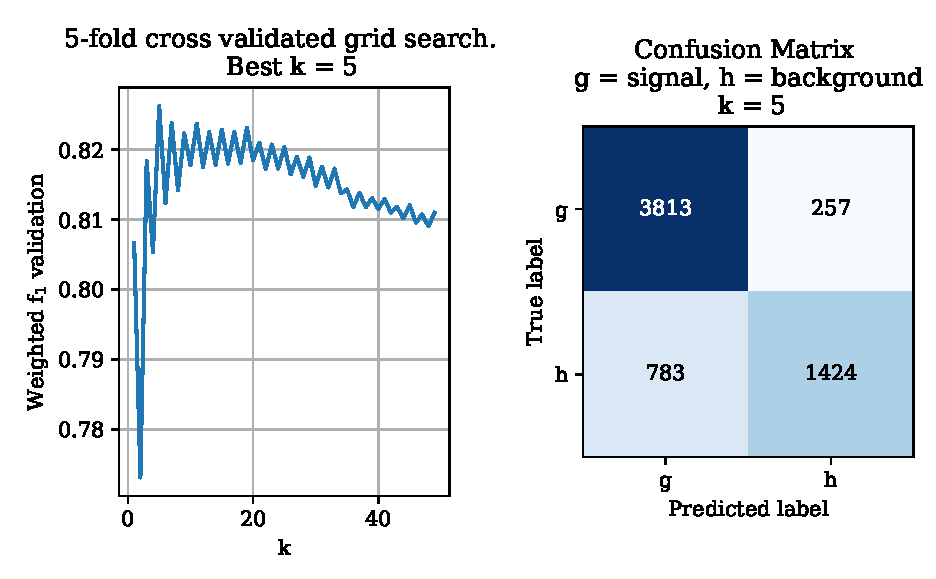
\includegraphics[scale=1]{{figures/kNN_cv_results}.pdf}
\caption{Results from tuned kNN using cross validation. The confusion matrix was
found using the test set.}
\label{fig:kNN}
\end{figure*}

\begin{figure}
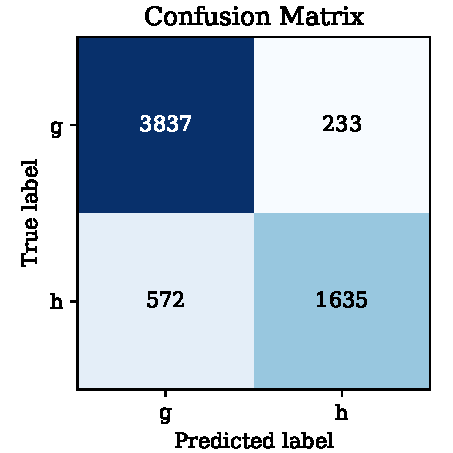
\includegraphics[scale=1]{{figures/nn_confusion_matrix}.pdf}
\caption{Confusion matrix of the neural network model applied to the test set.}
\label{fig:NN_confusion}
\end{figure}

\begin{figure}
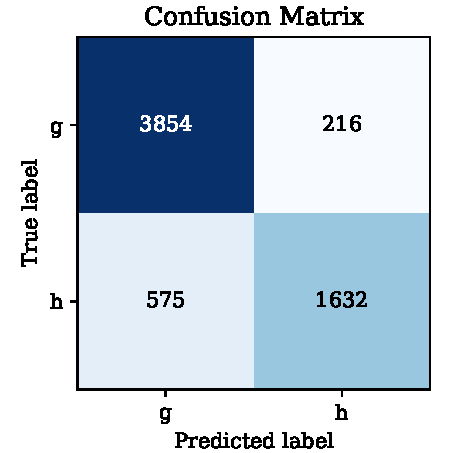
\includegraphics[scale=1]{{figures/xgboost_confusion_matrix}.pdf}
\caption{Confusion matrix of the gradient boosted model applied to the test set.}
\label{fig:XGB_confusion}
\end{figure}

\section{Discussion}
 
\section{Conclusion}


\section*{Acknowledgements}
We want to thank the University of California, Irving for providing us with the data used in this project.


%\bibliographystyle{iEEEtran}
\bibliography{bibliography}



\end{document}
